%!TEX root = Thesis.tex
\chapter{Layout-oriented Constraint Generation and Unification}\label{chap:cg}


  According to Figure~\ref{fig:LayoutFlow}, the constraint driven routing methodology attempts to generate the layout-oriented constraint groups in post-placement layout. In this section, we provide a flow to generate constraint group for routing purpose from required technology process rules, design guidelines and layout topology. 
  
  The detail flow of constraint group generation is shown in Figure~\ref{fig:LayoutCGGen}. From the beginning of our constraint group generation flow, we feed an analog layout design with cell location and connectivity informations into our constraint group generator. Our constraint group generation flow has three stages: Process rule constraint group generation, Pre-defined design guidelines constraint group generation and the Layout constraint extractor. The first stage is necessary, and the second is prior to the third one. In case there is no any constraints being applied in the second stage, this constraint generator tends to extract the constraint from existing layout. In other words, we value the designers' expertise in order to guarantee that the constraint driven routing methodology honors the routing priority as designers' expectation. Here we express the three steps of constraint generation in the following subsections. 
  
  \begin{figure}[t]
    \centering
      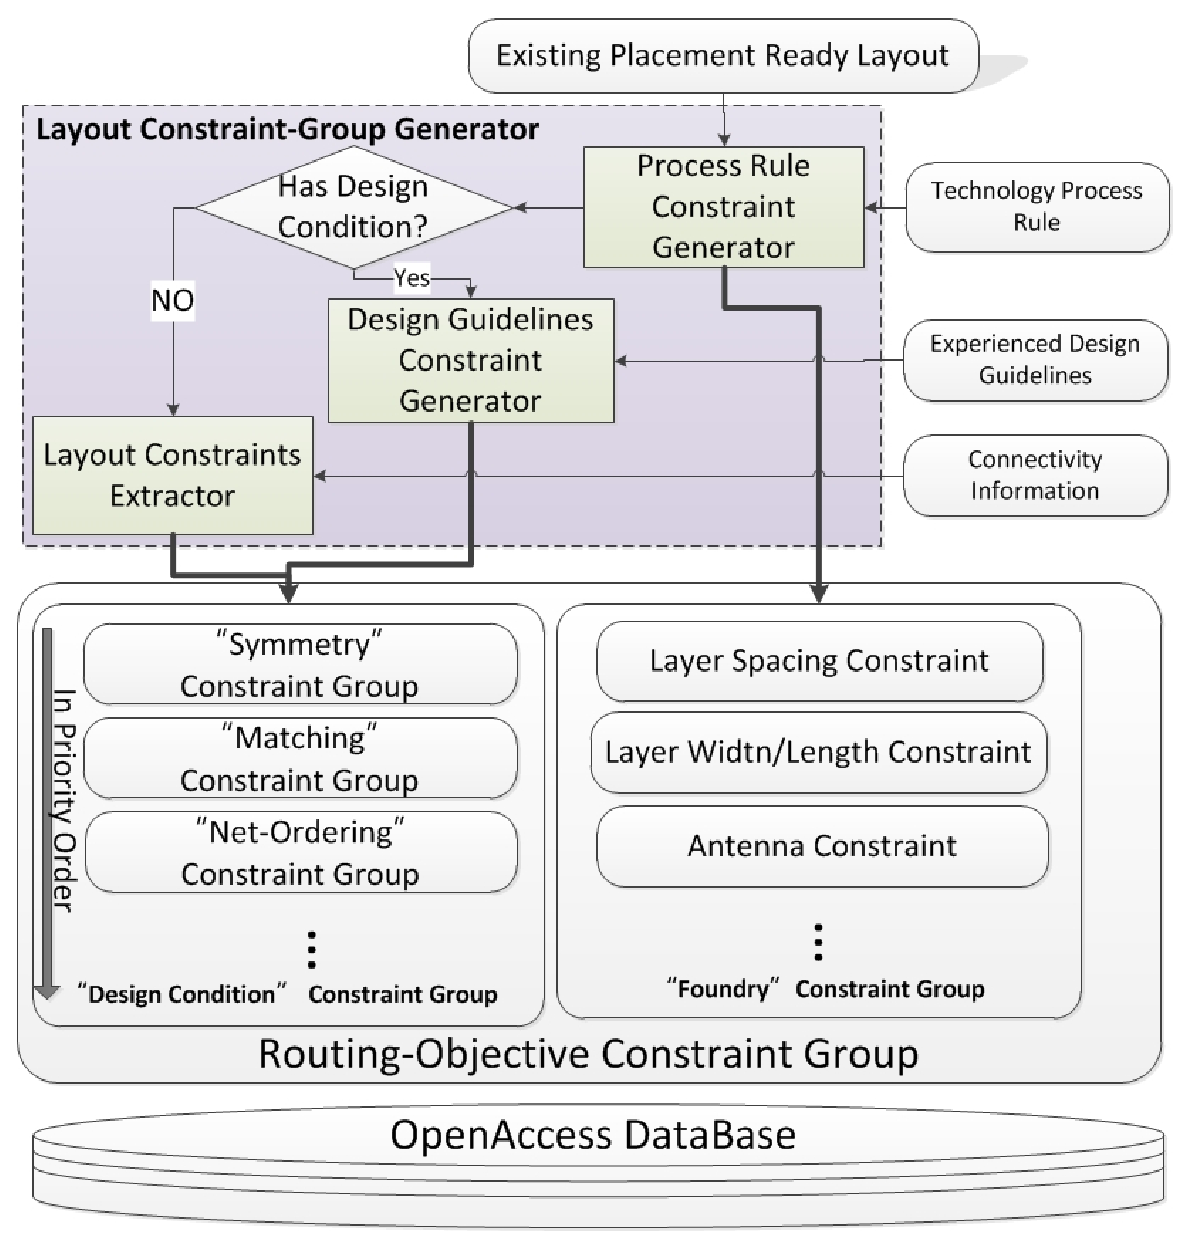
\includegraphics[width=0.5\textwidth]{Fig/CG/LayoutConGen.eps}
      \caption{Layout-oriented constraint generation flow.}
      \label{fig:LayoutCGGen}
  \end{figure}

  \section{Process Rules Constraint Group Generation}\label{sec:RCG}
  The ``foundry'' constraint group is automatically stored in the technology database under OpenAccess platform. Thus, applications developed on OpenAccess can access the foundry process rule directly before post-layout verification. In other words, the exact process rule can be considered during the placement and routing stage. Traditionally, works implement P\&R methodologies with abstract design ruls because it is complex and time-consuming to import the whole design rule of the target technology as constraints. Other than applying such abstract constraints, the mechanism of built-in constraint groups can check out the exact design rules at runtime stage. It indeed raises the efficiency with respect to fewer redesign cost. Most of the constraints for technology purpose are layer-related. Table~\ref{tableFoundryCon} expresses a group of layer constraints refering to a specific technology. However, according to rule complexity of advanced technologies, the built-in constraint group is inadequate for the new generation technology. 
  
  \begin{table}[ht]
    \centering
    \caption{Basic Foundry constraints}\label{tableFoundryCon}
    \begin{scriptsize}
      \begin{tabular}[t]{|l|l|}
        \hline
        Constraint Type & Value \\
        \hline
        minSpace  & ``METAL2'',0.16 \\
        \hline
        minEnclosure  & ``METAL2'',``VIA2'',0.01  \\
        \hline
        minEndofLineSpacing & ``METAL2'',0.1,0.1,0.42 \\
        \hline
      \end{tabular}
    \end{scriptsize}
  \end{table}
  
  
  \begin{figure}[t]
    \centering
    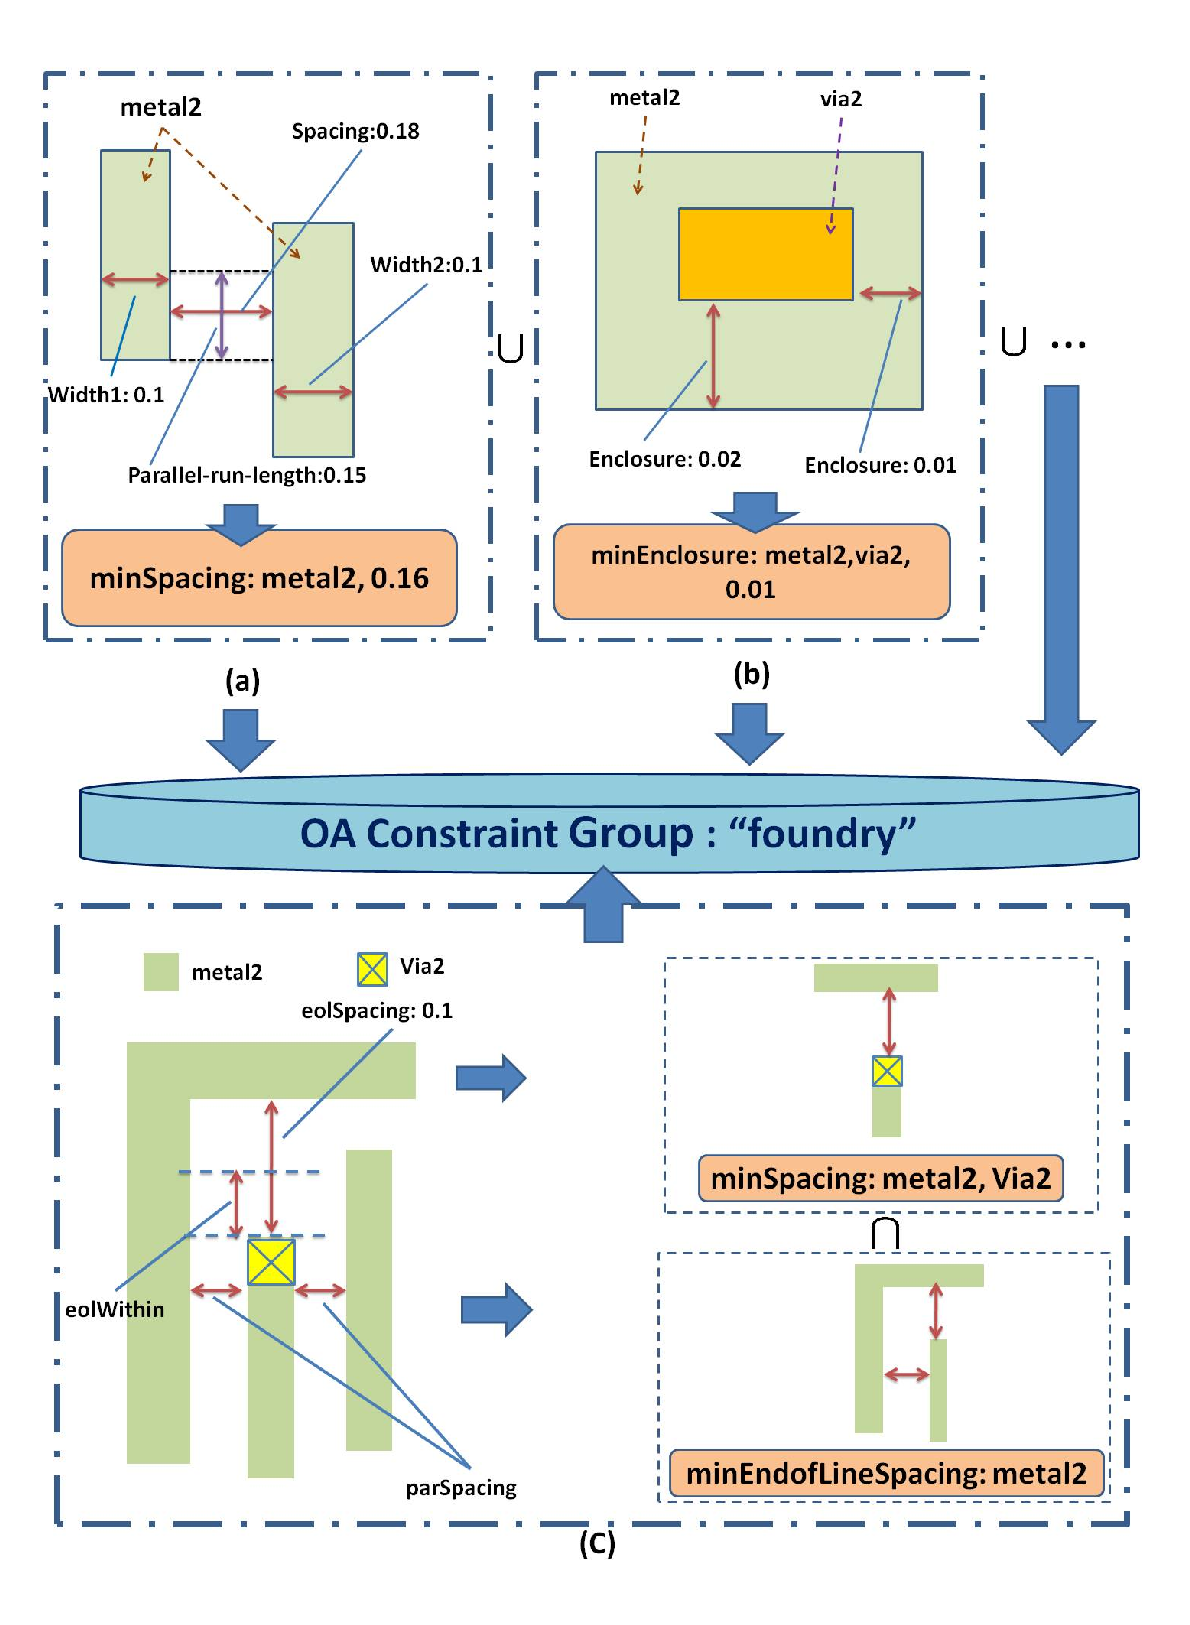
\includegraphics[width=0.5\textwidth]{Fig/CG/SimpleRuleCon2.eps}
    \caption{Mapping simple process rules to constraint group ``foundry''. (a) minimum spacing 0.16um on metal2. (b) minimum enclosure 0.01 with metal2 and via2. (c)Integration of minEndofLineSpacing and minSpacing to fulfill the rule.}
    \label{fig:SimruleCon}
  \end{figure}
  
  Fundamentally, OpenAccess constraint semantic supports basic geometric rules for a single layer or multiple layers. Figure~\ref{fig:SimruleCon}(a) shows a sample of minimum spacing of two shapes with the same metal, and we can also see minimum enclosure constraint that a layer(via2) is fully enclosed into another layer(metal2) in Figure~\ref{fig:SimruleCon}(b). It is feasible to transfer these kind of accurate process rules into constraint group.

  However, the basic geometric constraint type no longer satisfied the advanced technology process rule. Many conservative process rules are raised by the foundry due to DFM issues. Fortunately, the OpenAccess constraint group utility supports logical operation among constraints, which means that two or more constraints built-in constraints can form a harder constraint union. In Figure~\ref{fig:SimruleCon}(c), we can see that a process rule objective is to avoid violation that the minimum spacing between the end of a line from a via on a rectangle-shape metal and its neighbors. By logical interaction of basic physical constraints, minimum spacing to end-of-line (eol) for ``metal2'' and minimum spacing for ``metal2'' and ``via2'', the constraints exactly cover the rule which avoids violation.
  
  By a procedure of operation on transferring the process rules, the built-in constraint group of the foundry can be constructed.

  \section{Pre-defined Design Guidelines Constraint Group Generation}\label{sec:PreDesignCG}
  %According to Figure~\ref{fig:CG}, 
    Except the ``foundry'' constraint groups, each design can create their own custom constraint group with arbitrary semantics. Thus, two different circuit designs which share the same technology constraint group tend to preserve totally diversed constraint groups with distinct design purposes. Moreover, even dissimilar objectives are applied on the same analog design w.r.t. the same technology for particular performance requirement. Thus, the flexibility of user-defined constraint groups is important to have. 

    Traditionally, experienced analog designers manually annotate design constraints on the schematic view. The constraints are mostly related to performance intention, such as symmetrical constraints, proximity group and net ordering. Nevertheless, due to non-unified annotation, the instruction made by the designers cannot be exchanged with a general data model. Here we standardize aforementioned analog constraints into OpenAccess constraint format. 
  
    Other than extracting all the design conditions from an analog layout, we pick only symmetry and proximity constraints to demonstrate of user-defined constraint generation. According to strict hierarchy properties of analog design, if each element in the design has more than 2 constraints, the priority of these constraints is pre-defined by designers knowledge. Therefore, the constraint group can preserve not only the constraint type but also the hierarchical structure. Table~\ref{tableConType} shows the sample constraint type and value which can be preserved in OpenAccess constraint group data model. The constraint definitions below are symmetrical and matching constraints: 


    \newtheorem{Cons}{Constraint}
    \begin{Cons}
      {\bf MatchGroup}, a collection of cells which should be grouped in proximity. It defines the name of MatchGroup, and a series of names of cells.
    \end{Cons}
    \begin{Cons}
      {\bf SymGroup}, a symmetrical pair accompanied with a pre-defined symmetry line by SymLine constraint. The members of symmetrical pair can be cell name or group name defined by MatchGroup or other SymGroup name.
    \end{Cons}
    \begin{Cons}
      {\bf SymLine}, which shows the coordinate type and value of symmetry-axis for layout.
    \end{Cons}
  
  
    \begin{table}[ht]
      \centering
      \caption{Constraint sample type and value for layout design guidelines}\label{tableConType}
      \begin{scriptsize}
        \begin{tabular}[t]{|l|l|}
          \hline
          Constraint Type & Value \\
          \hline
          Symmetry Line & SymLine(name,axis-type,coordinate)  \\
          \hline
          Matching Group  & MatchGroup(name,list-of-cells)  \\
          \hline
          Symmetry Group  & SymGroup(name,Symline,pairs)  \\
          \hline
        \end{tabular}
      \end{scriptsize}
    \end{table}


    \begin{figure}[ht]
      \centering
        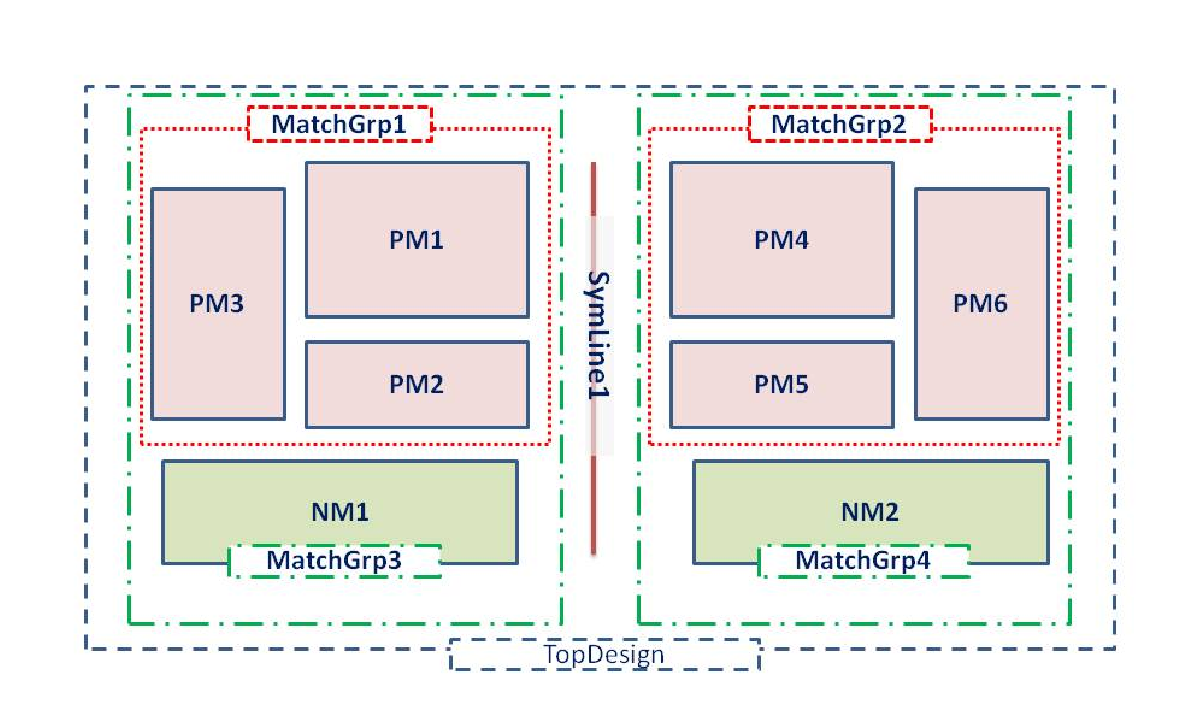
\includegraphics[width=0.7\textwidth]{Fig/CG/PreCG.eps}
      %\begin{spacing}{1}
      \begin{scriptsize}
      \begin{tabular}[t]{l}
        \toprule
      % \hline
        \multicolumn{1}{c}{Constraints in TopDesign}  \\
        \midrule
      % \hline
        SymLine(``SymLine1'',y,0) \\
      % \hline
        MatchGroup(``MatchGrp1'',(``PM1'',``PM2'',``PM3'')) \\
      % \hline
        MatchGroup(``MatchGrp2'',(``PM4'',``PM5'',``PM6'')) \\
      % \hline
        MatchGroup(``MatchGrp3'',(``MatchGrp1'',``NM1'')) \\
      % \hline
        MatchGroup(``MatchGrp4'',(``MatchGrp2'',``NM2'')) \\
      % \hline
        SymGrp(``SymGrp1'',``SymLine1'',(``MatchGrp3'',``MatchGrp4''))  \\
      % \hline
      \bottomrule
      \end{tabular}
      \end{scriptsize}
      %\end{spacing}
      \caption{Pre-defined Constraint Group with layout cell blocks illustration.}
      \label{fig:PreCG}
    \end{figure}
  
  
    We demonstrate the usage of constraint group in Figure~\ref{fig:PreCG} to annotate design conditions of layout. There are 8 cells including six PMOS and two NMOS in the layout. The pre-defined constraints are illustrated in the table of Figure~\ref{fig:PreCG} for layout at the top of Figure~\ref{fig:PreCG}. There are matching group, symmetry group and symmetrical line for symmetry constraint. The priority of constraints is flexible to decide. Here Figure~\ref{fig:PreCG} shows that matching group has higher ranking in constraint group. For example, PM2 is owned by ``MatchGrp1'' and ``SymGrp1'', but there is only a pair of cells or groups which can be a pair of each symmetry group in this format. We pick PM2 to be a child of  ``MatchGrp1'', then ``MatchGrp1'' is one of a child of ``MatchGrp3''. Therefore, ``MatchGrp3'' is symmetrical to ``MatchGrp4'' by ``SymLine1''. Finally, a group of constraints can exactly cover the symmetry and proximity constraints from design guidelines.


  \section{Layout Constraint Extraction}\label{sec:LayoutConExt}
    After extracting constraint rules from the process rules of the foundry, if there are no design guidelines left in the design, we attempt to extract constraints from the existing layout. Without the pre-defined constraint group generated in the previous step, our constraint extraction applies the methodology \cite{srm-massier-tcad08,palpndg-iccad2011}, shown in Figure~\ref{fig:CGExtract}. Here the extractor complies with the priority that matching constraint is precedential to symmetrical constraint. In the end, the extraction obtains the proximity and symmetry constraints from the layout after placement step. The constraint group generated by the extraction is similar to the pre-defined constraint group represented in Figure~\ref{fig:PreCG} with the same constraint order. Finally, we integrate these constraints into our hierarchical constraint group for constraint driven routing.
  
    \begin{figure}[ht]
      \centering
      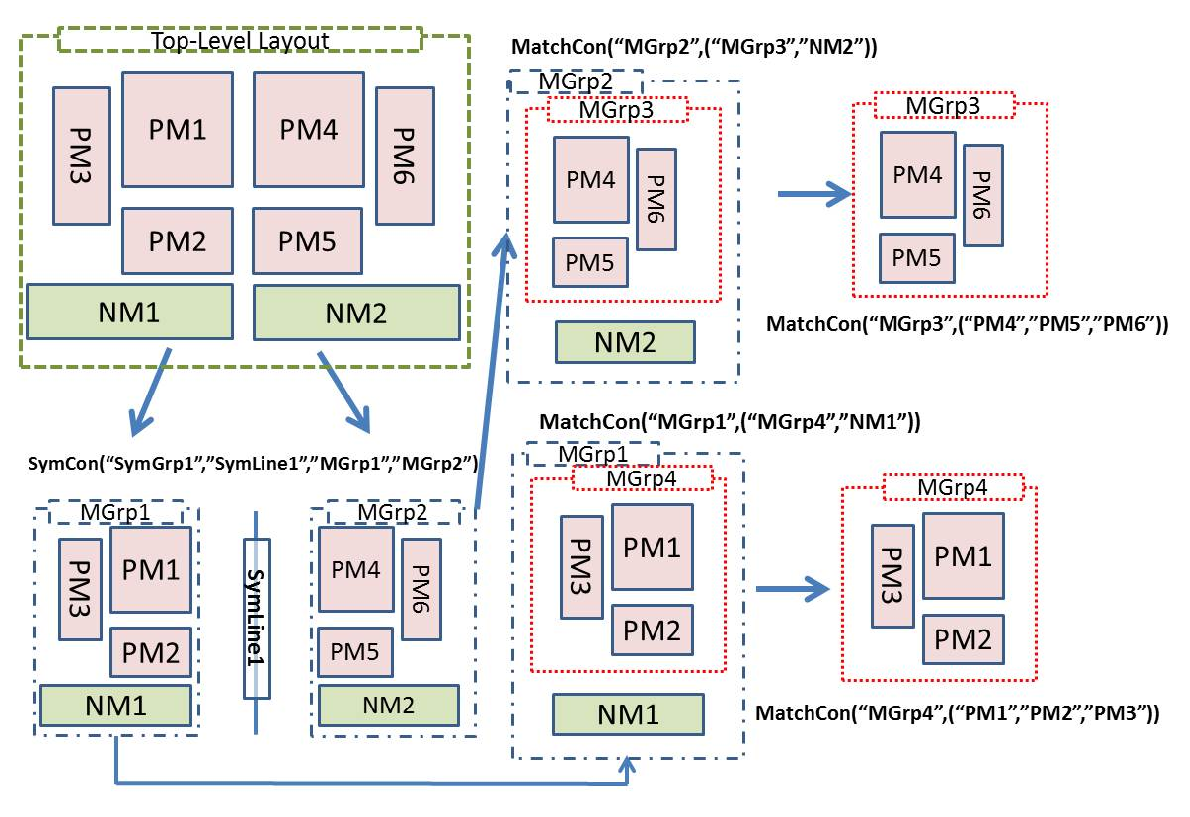
\includegraphics[width=0.7\textwidth]{Fig/CG/CGExtract.eps}
      \caption{Constraints extracted from the existing layout without pre-defined design conditions. The original top-level layout has PM1-PM6 and NM1,NM2. First of all, the top-level layout is divided into a symmetric pair with MGrp1 and MGrp2 via SymLine1. Recursively, MGrp1 and MGrp2 are partitioned in the sub-level. MGrp1 is separated as MGrp3 and NM2, and MGrp2 is separated as MGrp4 and NM1 similarly. In the bottom level, MGrp3 is consisted of PM4-PM6 and MGrp4 is consisted of PM1-PM3}
      \label{fig:CGExtract}
    \end{figure}



